\documentclass{article}
\usepackage[utf8]{inputenc}
\usepackage{graphicx}

\title{Reporte 1: Comparativa entre algoritmos de ordenamiento\\\textbf{Análisis de Algoritmos}}
\author{ Ramiro Estrada García\\2015190034 }
\date{17 de Noviembre del 2020}

\begin{document}
\maketitle
\vspace{5cm}
\section {Características del PC}
\begin{itemize}
	\item CPU: Intel Core i5 9700F a 4.1GHz
	\item RAM: 16GB a 2666MHz
\end{itemize}
\newpage
\maketitle
\section{Mejor caso}
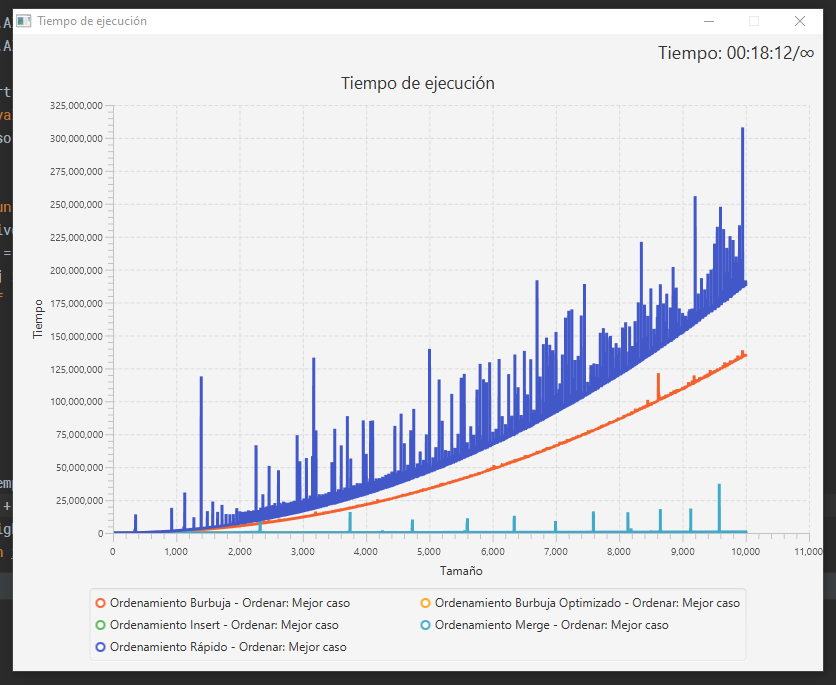
\includegraphics[width=12cm]{mejor.png}\\
En este caso, el Quick Sort tiene el peor rendimiento, siguiendole por el Burbuja. Los demás algorítmos, tuvieron un rendimiento 
lineal casi pegados al eje X. Esto demuestra que el QuickSort es ineficiente en el mejor de los casos.
\maketitle
\section{Medio caso}
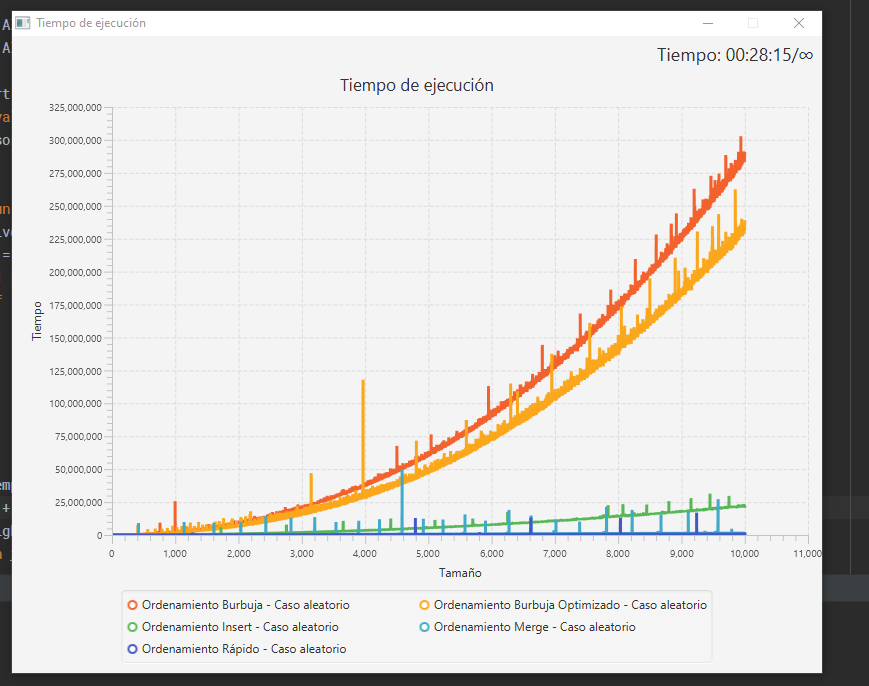
\includegraphics[width=12cm]{medio.png}\\
En este caso, los peores son el ordenamiento Burbuja y el Burbuja Optimizado. El Burbuja Optimizado trambién tiene un incremento 
cuadratico pero más aplanado que el Burbuja normal. Los demás tuvieron un incremento lineal muy reducido por lo que fuera de 
burbuja funcionan bien de manera general.
\maketitle
\section{Peor caso}
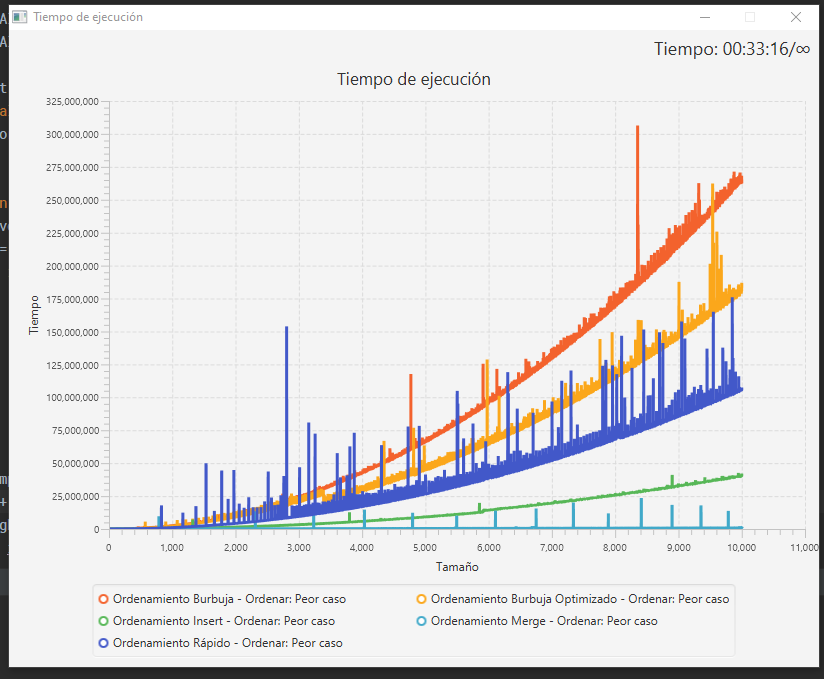
\includegraphics[width=12cm]{peor.png}\\
En este caso, se muestra que los burbuja tienen el peor rendimiento, el Quick y el Insert le siguien con un rendimiento aceptable
y terminamos con el merge sort que tiene un rendimiento lineal con la mayoria de los tamaños con muy poco tiempo.
\maketitle
\section{Mejor caso recursivos}
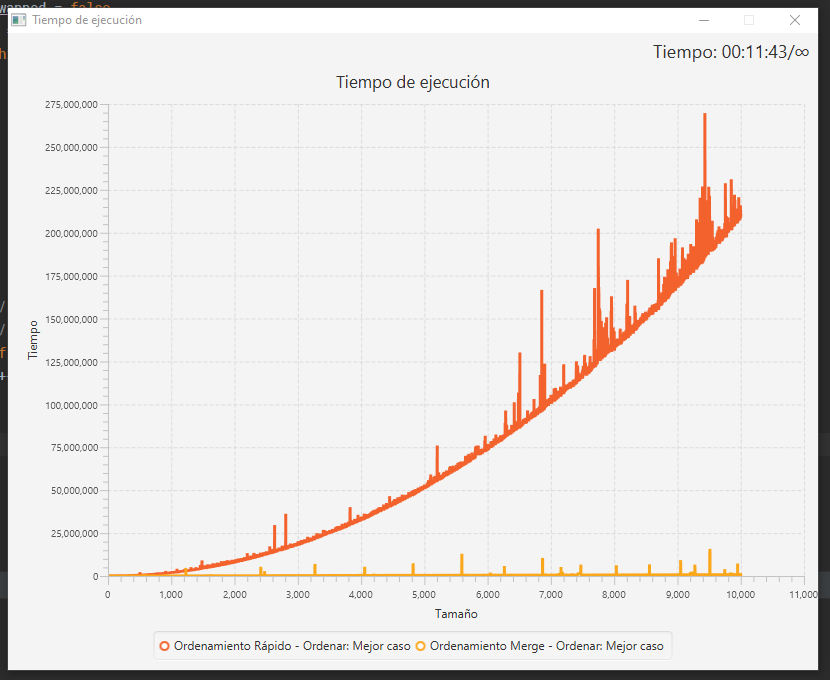
\includegraphics[width=12cm]{mejor_r.png}\\
En el mejor caso el Quicksort rinde muy mal en comparasion con el Merge teniendo un crecimiento cuadratico.
\maketitle
\section{Medio caso recursivos}
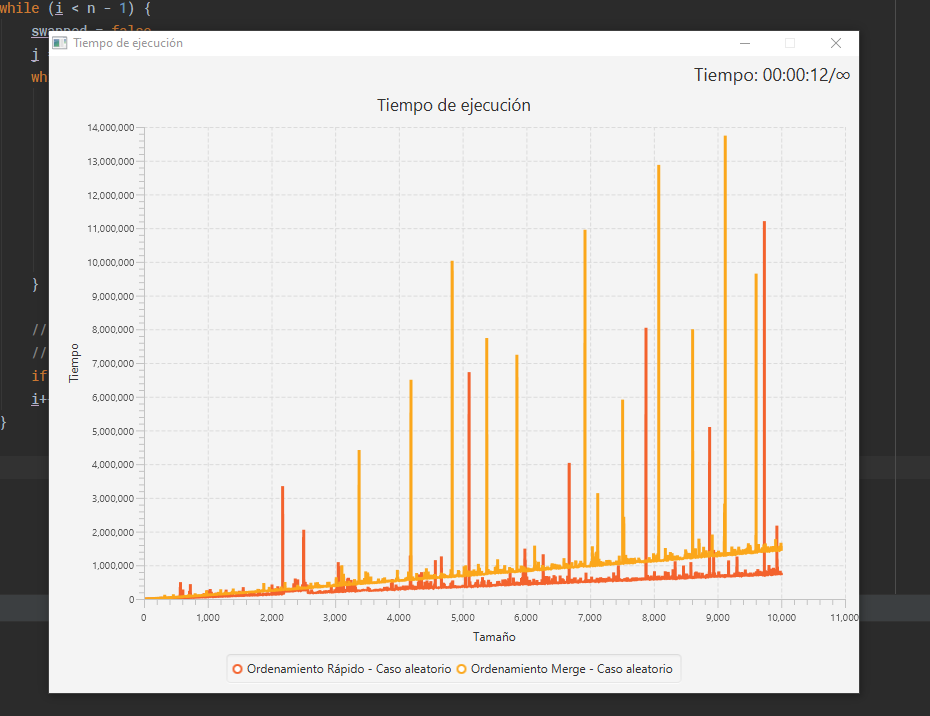
\includegraphics[width=12cm]{medio_r.png}\\
En el caso medio el Quick tiene un mejor rendimiento pero no esta muy alejado del Merge. Ambos tienen crecimiento lineal.
\maketitle
\section{Peor caso recursivos}
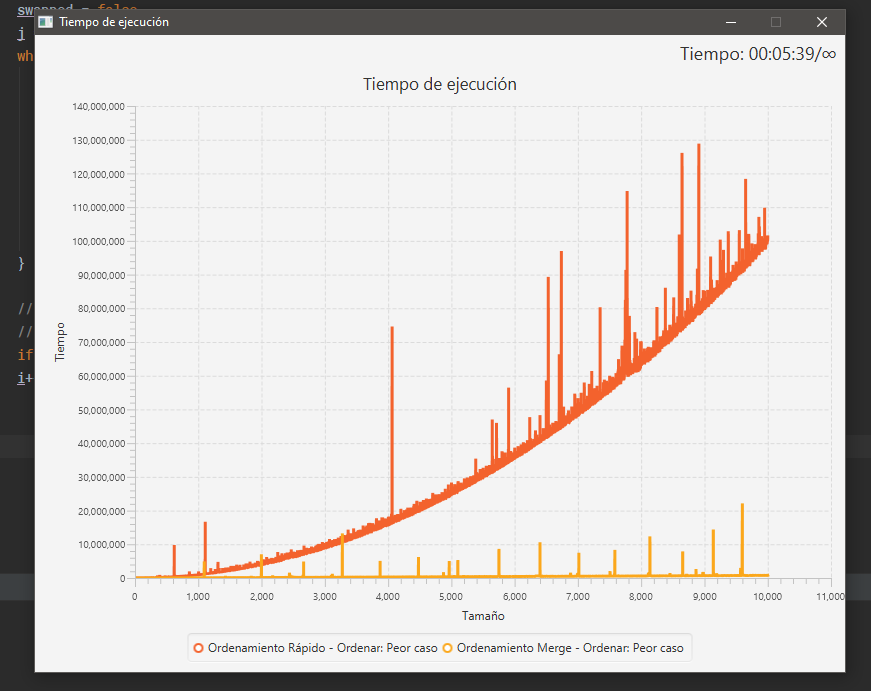
\includegraphics[width=12cm]{peor_r.png}\\
En el mejor caso el Quicksort rinde muy mal en comparasion con el Merge teniendo un crecimiento cuadratico.
\end{document}